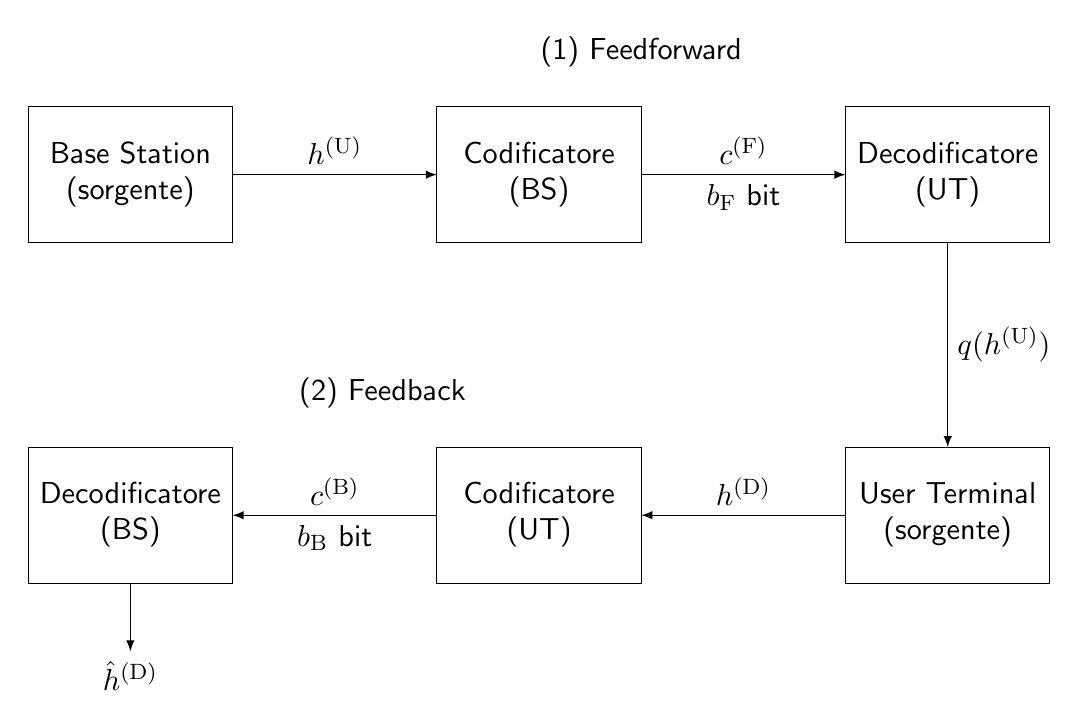
\begin{tikzpicture}[scale=0.865,>=latex]
    \tikzstyle{every node}=[font=\fontsize{11}{13}\sffamily]

    % Bottom Half

    \node at (5.2,2.8) {(2) Feedback};

    \draw[->] (1.5,0) -- (1.5,-1)
    node[below]{\(\hat{\bm{h}}^\mathrm{(D)}\)};

    \draw (0,0) rectangle (3,2)
    node[midway,align=center]{Decodificatore \\ (BS)};

    \draw[->] (6,1) -- (3,1)
    node[above,midway]{\(c^\mathrm{(B)}\)}
    node[below,midway]{\(b_\mathrm{B}\) bit};

    \draw (6,0) rectangle (9,2)
    node[midway,align=center]{Codificatore \\ (UT)};

    \draw[->] (12,1) -- (9,1)
    node[above,midway]{\(\bm{h}^\mathrm{(D)}\)};

    \draw (12,0) rectangle (15,2)
    node[midway,align=center]{User Terminal \\ (sorgente)};

    % Top Half

    \node at (9,7.8) {(1) Feedforward};

    \draw[->] (13.5,5) -- (13.5,2)
    node[right,midway]{\(q(\bm{h}^\mathrm{(U)})\)};

    \draw (12,5) rectangle (15,7)
    node[midway,align=center]{Decodificatore \\ (UT)};

    \draw[->] (9,6) -- (12,6)
    node[above,midway]{\(c^\mathrm{(F)}\)}
    node[below,midway]{\(b_\mathrm{F}\) bit};

    \draw (6,5) rectangle (9,7)
    node[midway,align=center]{Codificatore \\ (BS)};

    \draw[->] (3,6) -- (6,6)
    node[above,midway]{\(\bm{h}^\mathrm{(U)}\)};

    \draw (0,5) rectangle (3,7)
    node[midway,align=center]{Base Station \\ (sorgente)};
\end{tikzpicture}
